\begin{frame}{Motivation for a categorical classification}
    \begin{block}{Underlying problem}
        \begin{itemize}
            \item Treating tZq as background lead to heavy missclassification
            \item Giving tZq a different training label should decrease the problem
        \end{itemize}
    \end{block}
    \begin{block}{Technicalities}
        \begin{itemize}
            \item Use OneHotEncoding to give labels to signal, background and tZq
            \item Plot response and ROC for every label separately
            \item The final response is a vector. One component per label likelihood
            \item All components add up to 1 
        \end{itemize}
    \end{block}
\end{frame}

\begin{frame}{Previous results}
    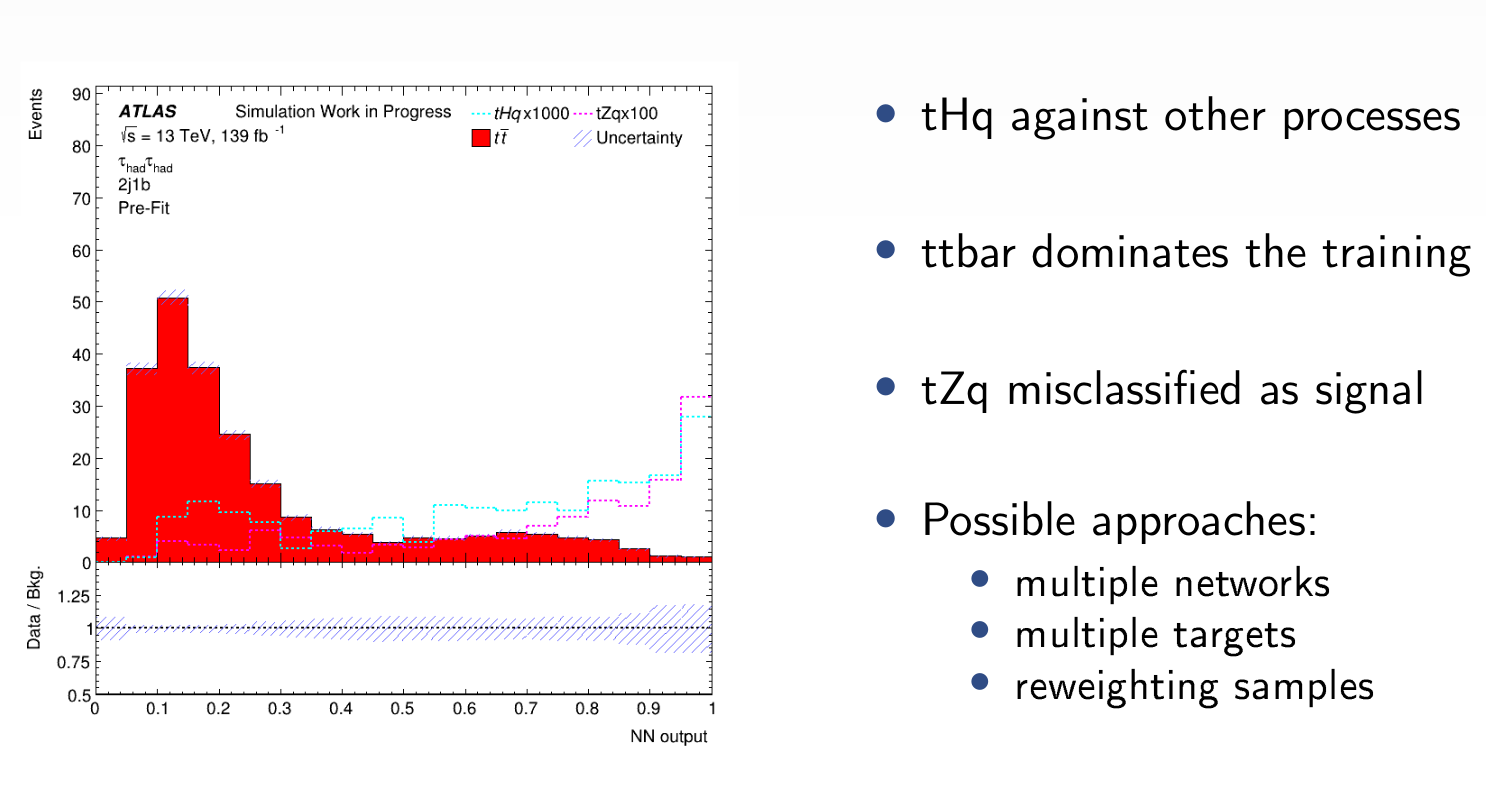
\includegraphics[width=\textwidth]{beforeCat}
\end{frame}

\begin{frame}{Response plot}
    \centering 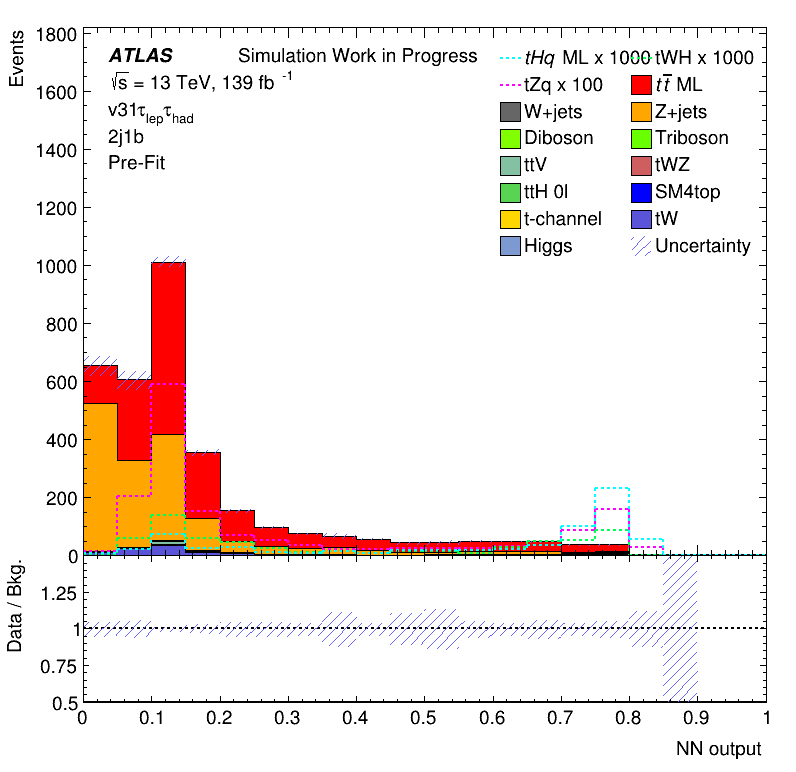
\includegraphics[width=0.6\textwidth]{lephad_cat.png}
    \begin{itemize}
        \item Majority of \tZq is no longer missclassified
        \item Part of \tZq is still missclassified but \tHq also gets a cleaner peak
    \end{itemize}
\end{frame}